% !TeX root = ../main.tex

\chapter{基于时间序列异常检测的根因分析系统设计与实现}
\label{cha:intro}
\section{问题描述}
在复杂系统中,无论是微服务还是云网络的场景,一方面,我们会得到单点的多个指标数据,也就是单个点上多条时间指标序列,而且由于可能是不同类型的点(例如微服务中的操作系统、数据库、容器、中间件以及云网络中的网关、交换机、虚拟机、物理机等),其指标也未必是同一个集合。另一方面,复杂系统中当出现异常时异常会在异常中蔓延,通常通过调用服务的方式来传播,本文中我们认为这种边是已知的。然后在具体的问题中,通常我们会有一个得知整个系统是否发生故障的入口,然后在这个时间点,有可能有多个点以及多条链路发生故障,我们需要快速定位到是哪个节点最初发生故障并通过各种方式传播到了整个系统导致系统整体运行出现问题。

本文以2020AIops挑战赛《微服务应用系统故障发现和根因定位》进行复杂系统的根因分析系统设计与实现的工作。比赛中我们得到了所有节点包括操作系统、容器和数据库的单点信息,并且得到了不同节点之间调用服务的记录。其中包括所有节点及其静态拓扑图如图~\ref{fig:static_topo}所示。我们会得到若干个时间段,表示在这个时间段上整个系统出现了问题。问题分为网络故障和节点故障,节点故障需要我们给出某个节点的某个指标,而网络故障如果在操作系统上需要给出指标,否则只需要定位到节点即可。

\begin{figure}[htbp]
    \centering
    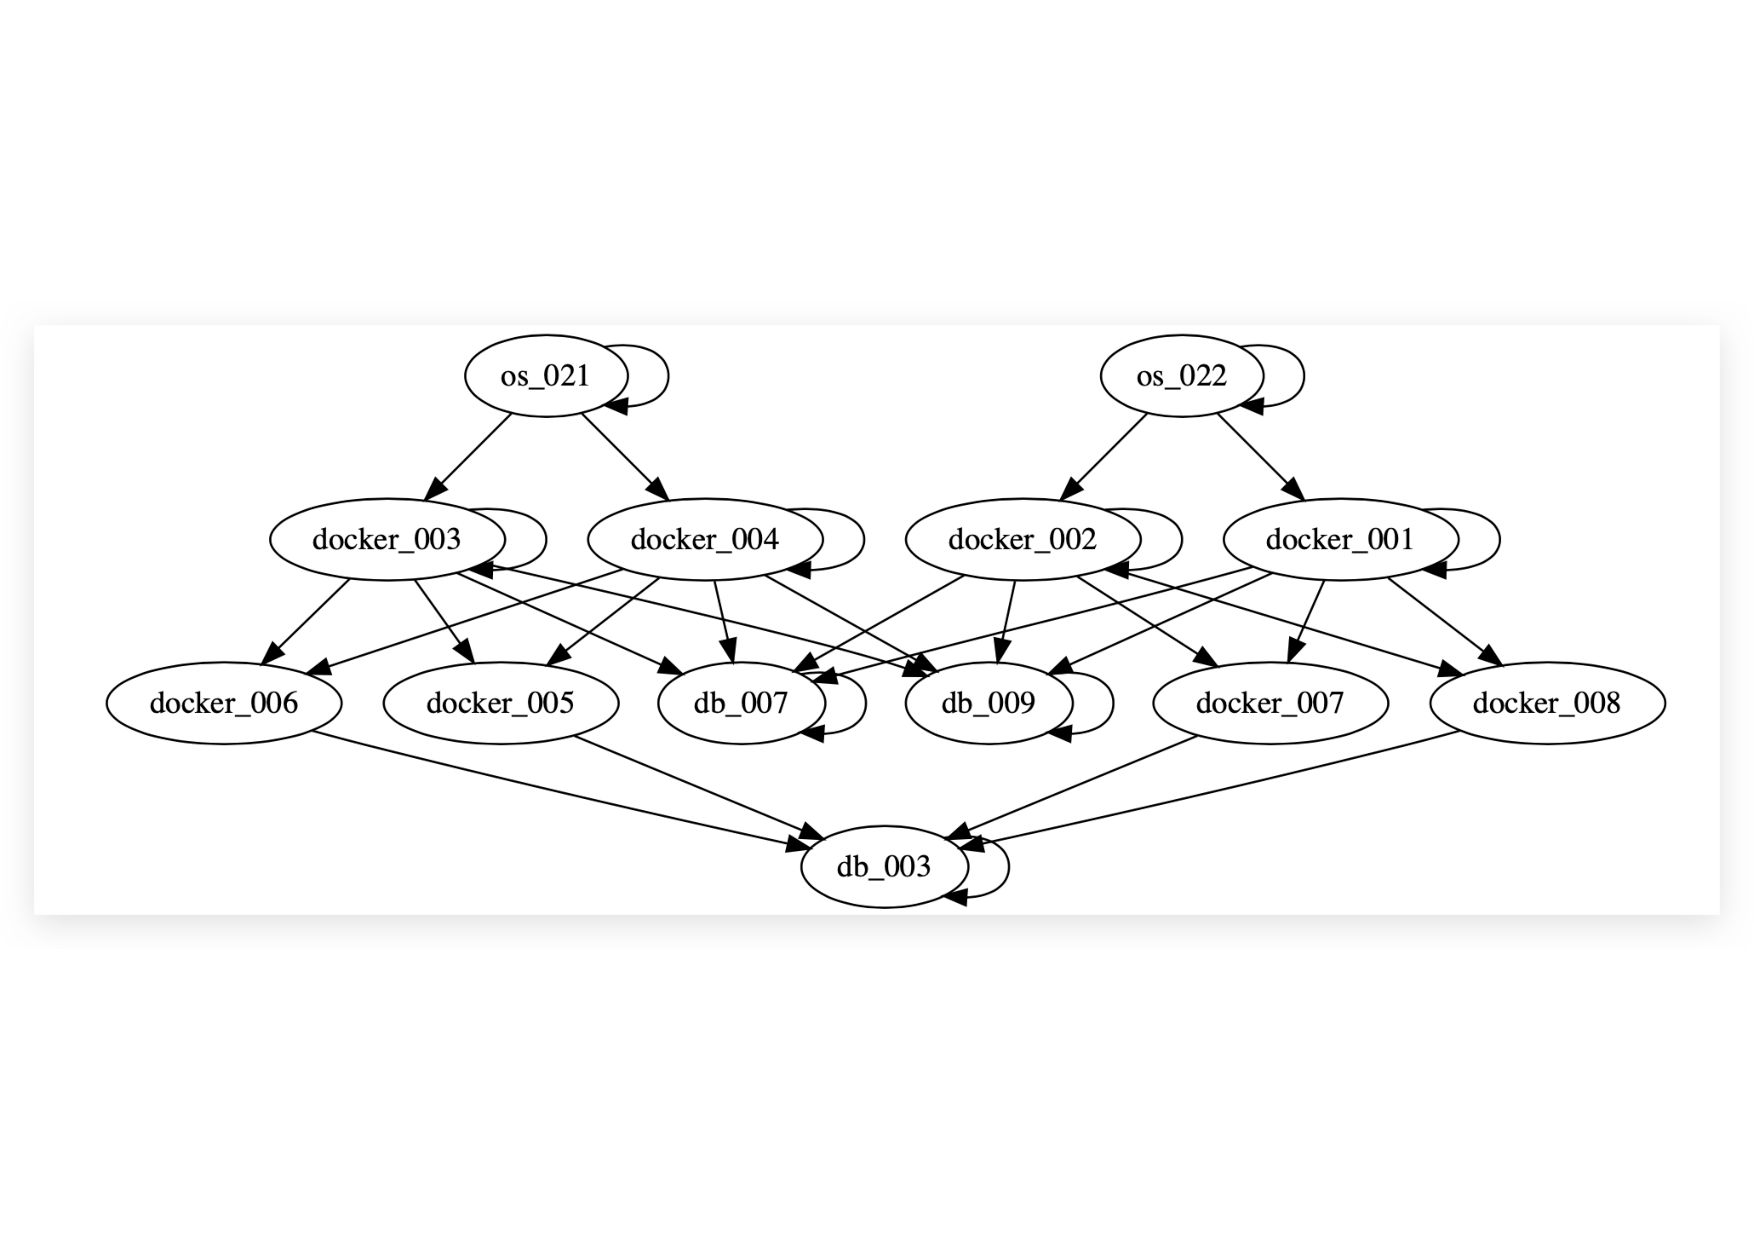
\includegraphics[width=\textwidth]{static-topo.pdf}
    \caption{静态拓扑图}
    \label{fig:static_topo}
  \end{figure}

\section{框架设计}
本文设计的根因分析框架如图~\ref{fig:part2-overview}所示:
\begin{figure}[htbp]
    \centering
    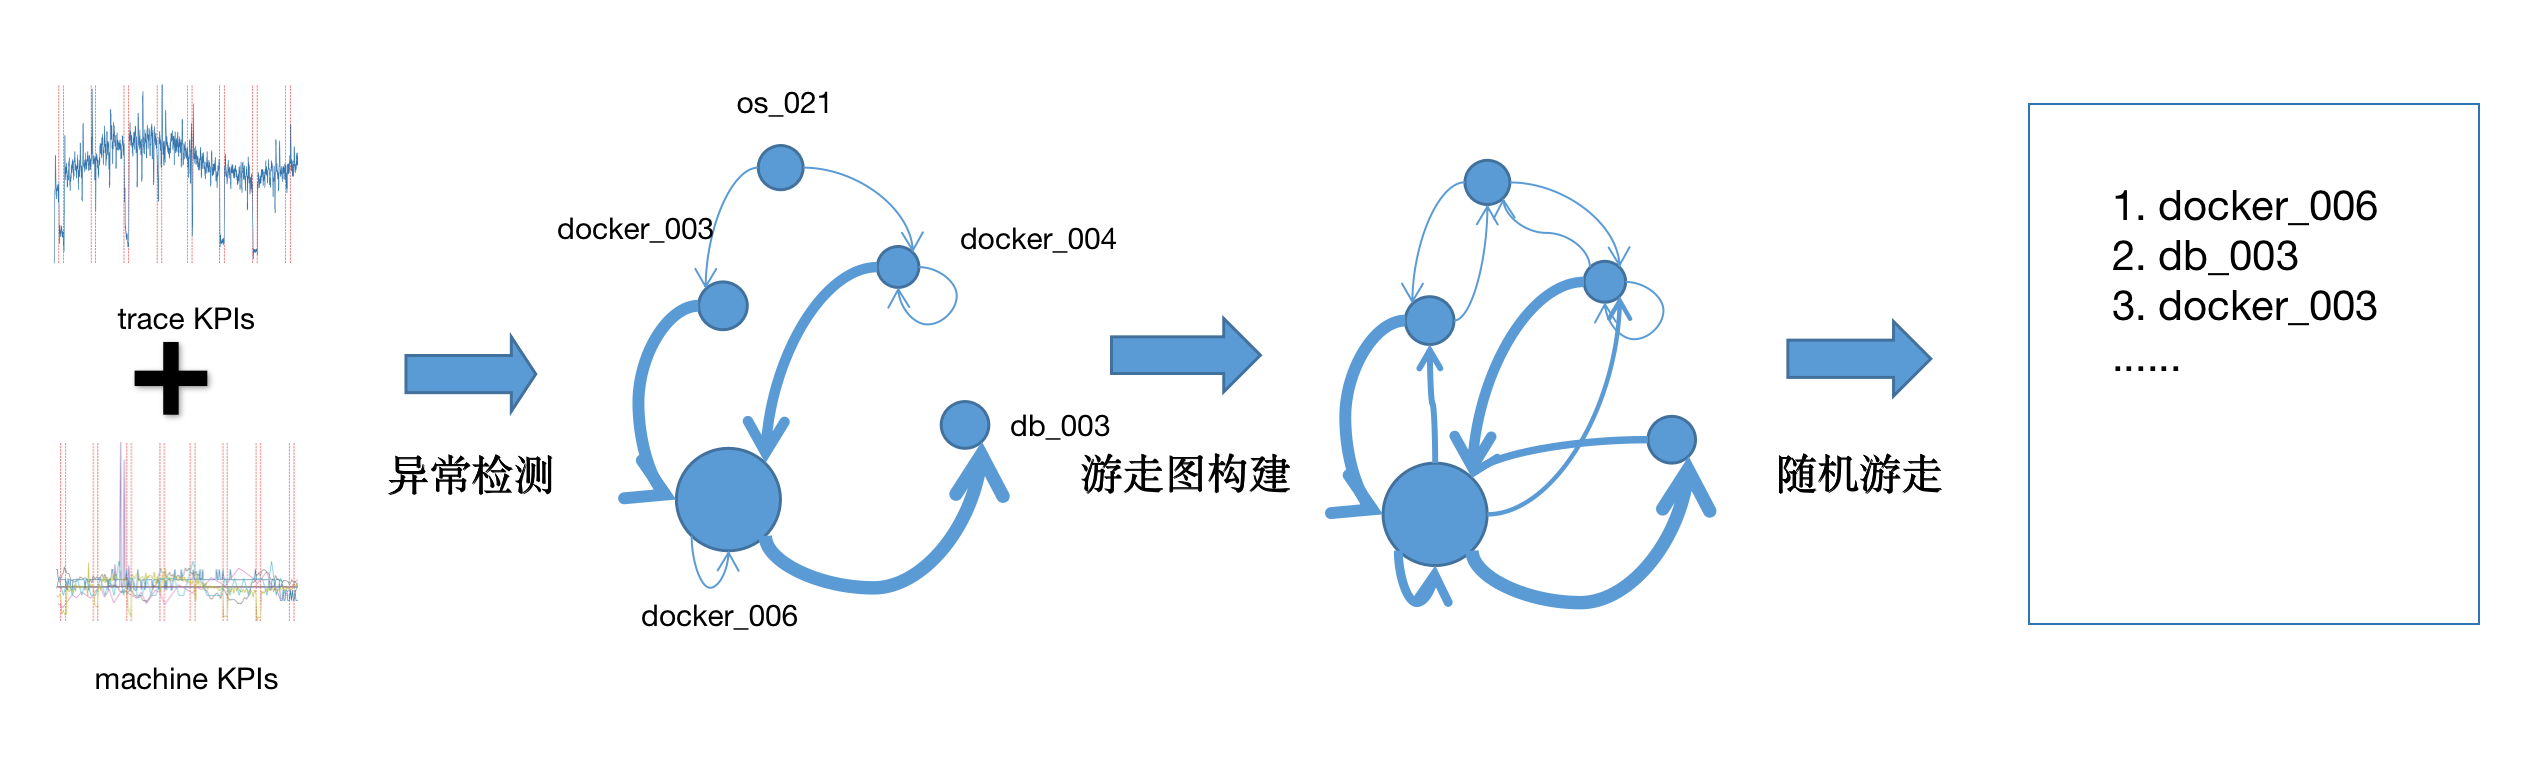
\includegraphics[width=\textwidth]{part2-overview.png}
    \caption{基于时间序列异常检测的根因分析系统框架}
    \label{fig:part2-overview}
  \end{figure}

首先我们通过预处理可以得到一系列节点上的KPI和节点之间调用服务的相关指标(例如调用次数、延迟等),通过对这些KPI运行异常检测算法我们得到这些曲线的异常分数,并将其画到图上,当一个点的指标表现越异常,,它的节点半径越大,同时如果一条边越异常,那么这条边就越粗。然后我们通过在边上添加一些边或者修改一些边的权重得到一张随机游走图。最后在图上运行一个随机游走算法来得到最有可能是根因的节点结果,然后再进一步定位到节点的指标。接下来详细介绍各部分实现的细节。
\section{异常检测模块}
在异常检测模块,我们期望在每个故障的时刻给出每条时间序列数据的异常程度,然后再用某个聚合函数(例如max)将多条时间序列数据的分数变成单点/边的异常分数。由于单一时间序列数据得到的采样点最多只有300余个,无法使用基于深度学习的算法。因此我们需要用一些比较传统的方法,本文中我们选择了KDE算法,因为其计算简单、通用性强,适用于各种特性的KPI。但因为数据中存在明显的突刺(可能是统计错误)和周期性问题会影响到KDE算法的正确性,因此我们先将明显的突刺去掉,以及减去周期性的数据。其次,不同的时间序列数据可能具有不同的量纲和数量级。当各个数据之间差异很大的时候,直接用原数据做异常检测进行分析的话,就会突出数值较高的指标在综合分析中的作用,而削弱数值低的指标的作用。为了将所有时间序列数据的异常分数放在一起比较的结果具有可靠性,我们需要先将所有数据做归一化、总结如下:第一步做归一化,第二步去掉尖刺数据,第三步进行周期性检测,将周期性数据从原数据中减掉,最后一步进行KDE异常检测。
\subsection{归一化}
目前常用的数据归一化方法主要是min-max和z-score标准化,考虑到min-max受异常值影响较大,我们采用了z-score标准化的方法。设原始数据的值为$x_i$,$mean$为原始数据的平均值,$std$为原始数据的标准差,则:
\begin{equation}
y_i = \frac{x_i-mean}{std}
\end{equation}

$y_i$为归一化后的数据,均值为0,方差为1,而且没有量纲。
\subsection{去除尖刺}
去除尖刺的目的是为了消除统计错误,也就是数据中明显不符合正常数据的凸起。但我们不能采用将边缘的极值去掉的方法,因为我们想要检测的异常可能就是处于边缘的极值,但是这种异常和统计错误的区别就是持续时间会相对久一些(例如5分钟以上),我们针对做以下平滑的方式:
\begin{equation}
z_i = \begin{cases} \frac{y_{i-1} + y_{i+1}}{2}, & (y_i - y_{i-1} > th \& y_i - y_{i+1} > th) | (y_{i-1} - y_i > th \& y_{i+1} - y_i > th) \cr y_i, & otherwise  \end{cases}
\end{equation}

$z_i$则为去除尖刺后的数据。
图~\ref{fig:smooth}展示了一个去除突刺的示例。其中红色标红的是出现故障的区间,如果不去除这些尖刺可能会导致在计算KDE时将尖刺统计在内而出现问题,0:45左右是真正出现故障的时间,而其他时间的波动都是正常波动,而去除尖刺之后我们很好地保留了真正的故障时段的异常,而去除了其他时刻的尖刺,保证其他时刻不会被误报。

\begin{figure}[htbp]
  \centering
  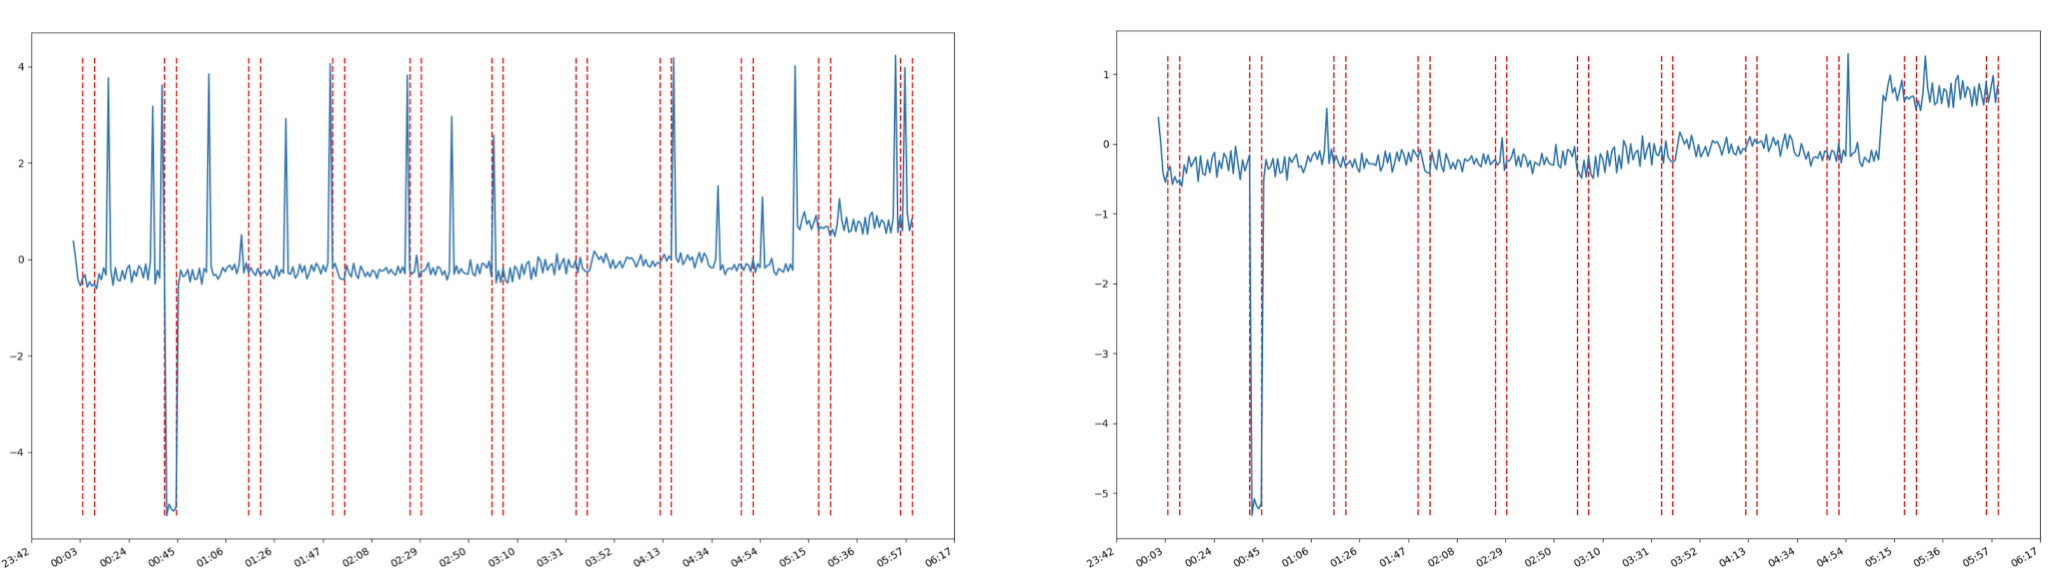
\includegraphics[width=\textwidth]{smooth.png}
  \caption{去除尖刺示例}
  \label{fig:smooth}
\end{figure}
\subsection{周期性数据去除}

在实际KPI中我们经常会遇到如~\ref{fig:period:left}所示的数据,具有很强的周期性,
这样的数据完全是符合历史特征的,所以不应该被判断为异常。但如果我们用KDE算法的话,一个前提是当前数据只和周围数据相关,不会考虑到很久以前的数据,所以我们需要把周期性先给去掉。那么首先我们就要知道序列的周期是多长,这里我们用了自相关函数的方法,计算方法为:
\begin{equation}
  acf_i = \sum_{j=1}^{N-i}z_j\times z_{j+i}
\end{equation}

$acf$函数如图~\ref{fig:period:middle}所示,然后我们从画出的自相关函数图中就可以确立出函数的最小正周期是120,然后我们再统计出周期内每个位置的平均数据,并且用原数据的每个位置减去他们在周期中所处位置平均值得到处理好的数据如图~\ref{fig:period:right}所示,可以看到大部分尖刺都被去掉,也不会出现预期之外的异常。
\begin{figure}[htbp]
    \begin{minipage}[t]{0.33\linewidth}
    \centering
    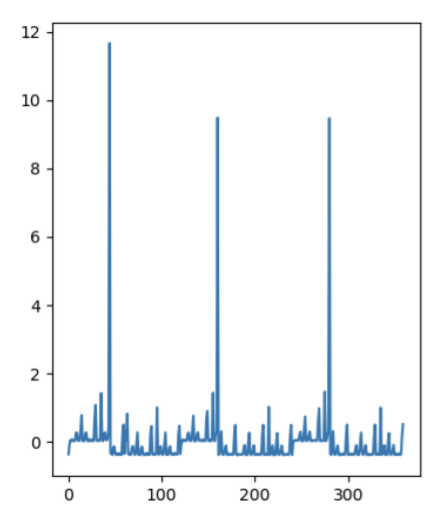
\includegraphics[width=\textwidth]{period_left.png}
    \caption*{(a)原始数据}
    \label{fig:period:left}
    \end{minipage}
    \begin{minipage}[t]{0.33\linewidth}
    \centering
    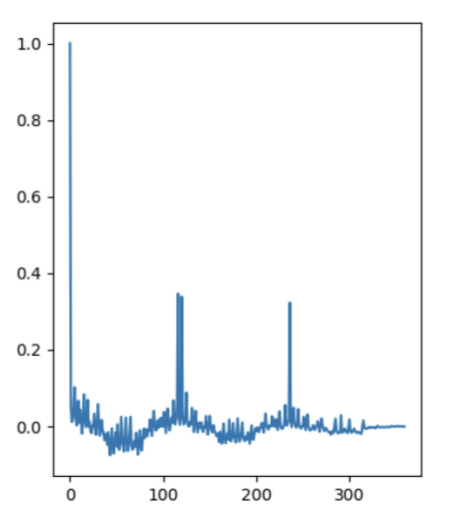
\includegraphics[width=\textwidth]{period_middle.png}
    \caption*{(b)自相关函数}
    \label{fig:period:middle}
    \end{minipage}
    \begin{minipage}[t]{0.33\linewidth}
      \centering
      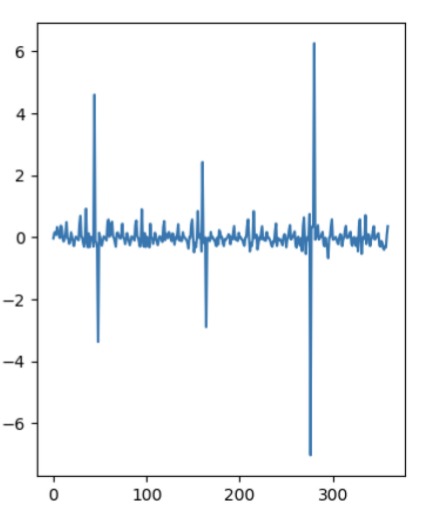
\includegraphics[width=\textwidth]{period_right.png}
      \caption*{(c)去除周期后的数据}
      \label{fig:period:right}
      \end{minipage}
    \caption{对数据去除周期化的过程}
\end{figure}
\subsection{KDE异常检测}
KDE是概率论中用来估计未知函数密度的非参数检验的方法之一,可以根据观察到的样本来估计随机变量的概率密度函数。
\begin{equation}
\hat{f}(x) = \frac{1}{n}\sum_{i=1}^nK(x;x_i)
\end{equation}
$K$是核函数,有多种选择,本文中我们采用了高斯核函数,$n$则是采样个数。KDE的核心思想就是对每个采样点形成一个一定带宽的核函数然后将所有采样点的核函数叠加起来即可,本文采取的带宽为0.4。当有了随机变量的密度函数之后,我们就可以用来计算新出现的数据概率了。本文中我们发现故障的持续时间总是5分钟,当给出故障时间点时,我们用前15分钟的数据来估计出一个密度函数,然后再来评估故障发生之后5分钟内数据出现的概率,概率越低说明这段时间的数据越异常,那么异常分数就越高。
\section{根因分析模块}
在异常检测模块,我们得到了每条曲线在该时刻的异常分数,对于一个点来说,我们认为他的异常分数就是所有曲线的异常分数的最大值,对于一条边来说,我们认为他的异常分数是所有边上的曲线分数的异常分数的平均值。因为单条边的分数具有偶然性。因此我们可以得到了如图~\ref{fig:error:example}所示的故障示例,其中点的大小代表点的异常分数的大小,而边的粗细代表边的异常程度的大小。
\begin{figure}[htbp]
  \centering
  \begin{subfigure}[b]{\textwidth}
    \begin{minipage}[t]{0.5\linewidth}
      \centering
      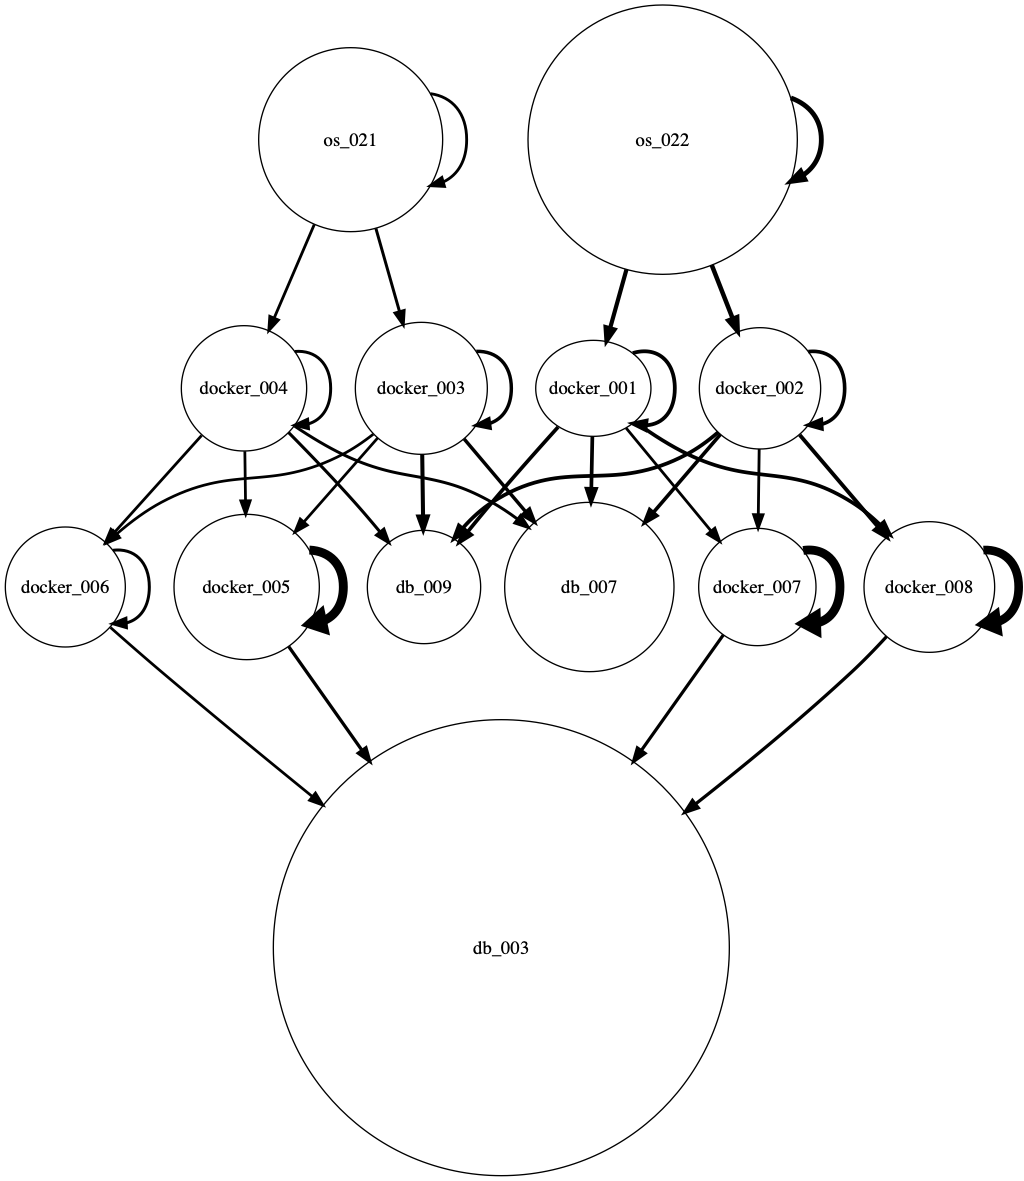
\includegraphics[width=\textwidth]{db_error.png}
      \caption{db故障}
      \label{fig:error:db}
    \end{minipage}
    \begin{minipage}[t]{0.5\linewidth}
      \centering
      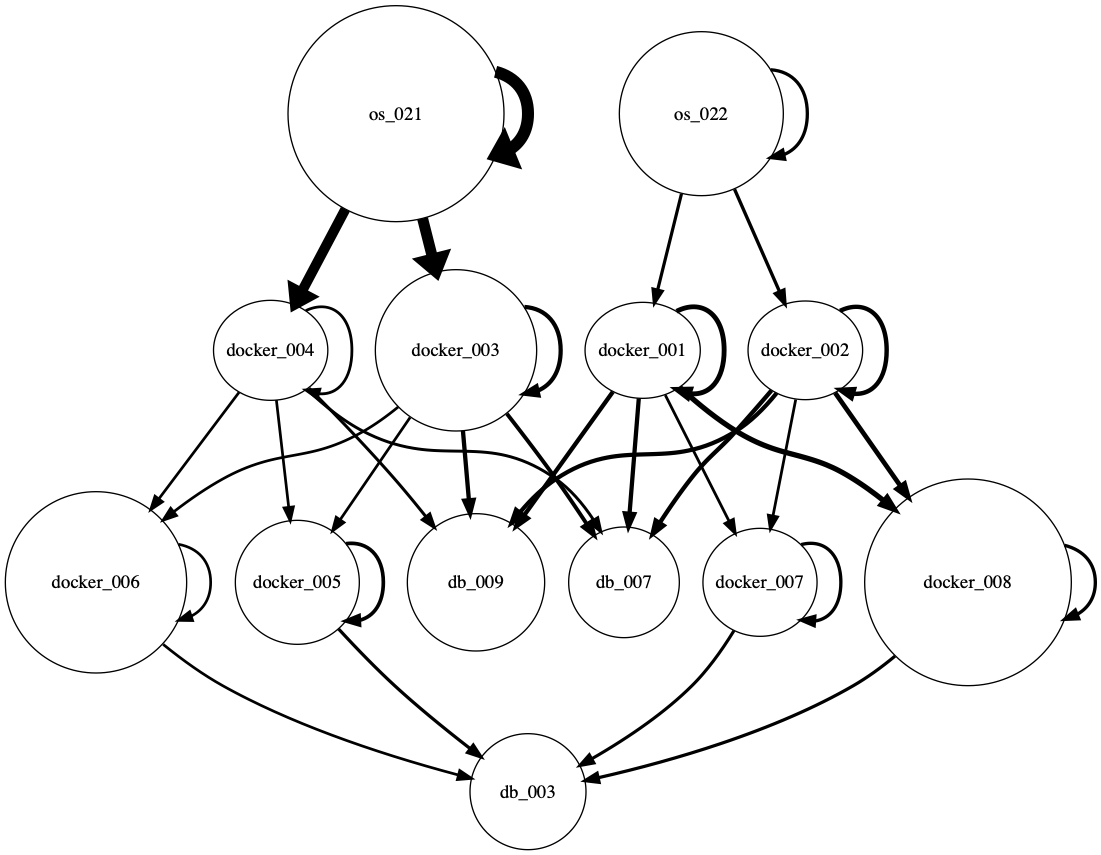
\includegraphics[width=\textwidth]{os_error.png}
      \caption{os故障}
      \label{fig:error:os}
    \end{minipage}
  \end{subfigure}

  \begin{subfigure}[b]{\textwidth}
    \begin{minipage}[t]{0.5\linewidth}
      \centering
      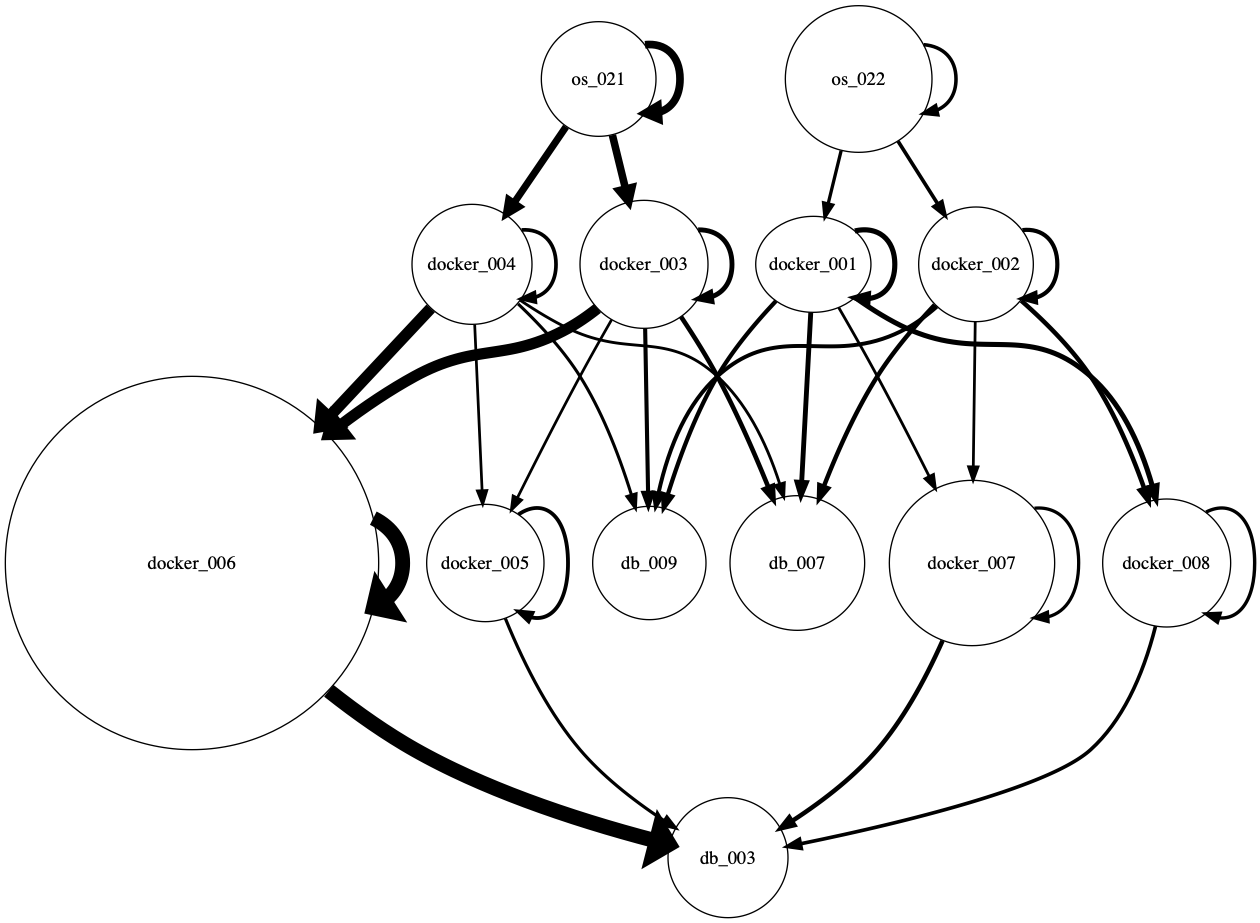
\includegraphics[width=\textwidth]{docker_cpu_error.png}
      \caption{docker cpu故障}
      \label{fig:error:db}
    \end{minipage}
    \begin{minipage}[t]{0.5\linewidth}
      \centering
      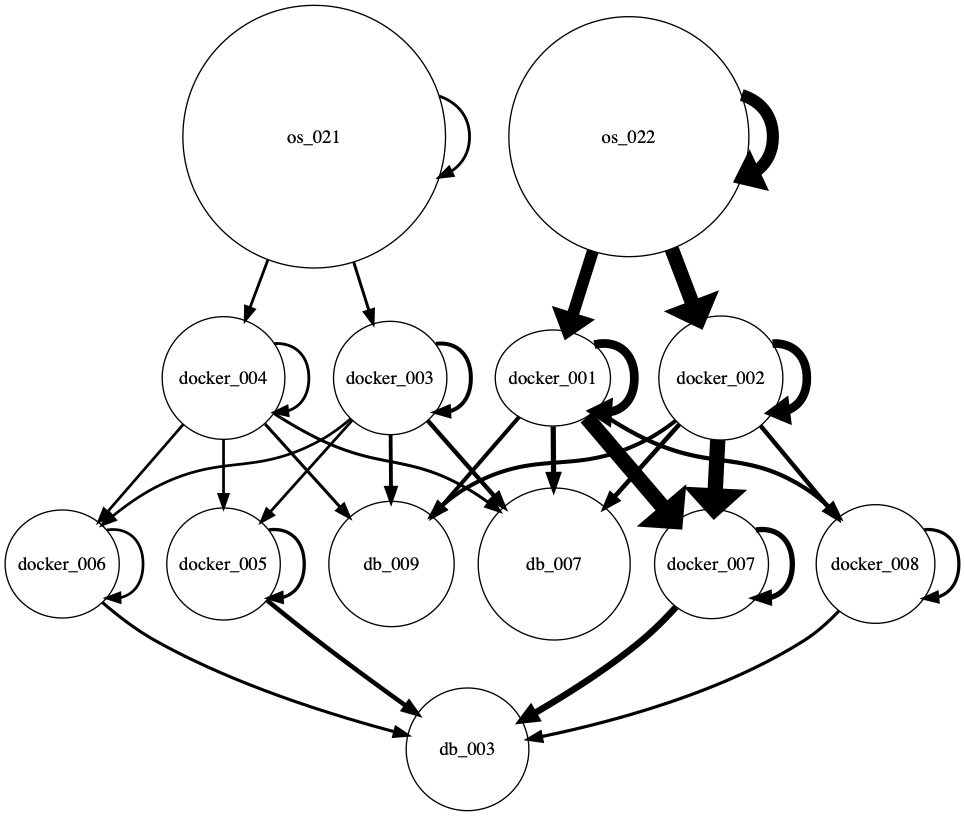
\includegraphics[width=\textwidth]{docker_network_error.png}
      \caption{docker 网络故障}
      \label{fig:error:os}
    \end{minipage}
  \end{subfigure}
  \caption{AIOPS2020挑战赛中故障示例}
  \label{fig:error:example}
\end{figure}
\subsection{构建随机游走图}
我们要在原先的异常图的基础上构建随机游走图。不妨认为节点为1到N,然后node\_score[i]表示i的异常分数,而edge\_score[i,j]表示(i,j)边的异常分数。不同于之前的工作,我们直接将服务调用时间的异常分数作为边的权值,因此我们需要以下三种边:
\begin{itemize}
  \item 前向边:为了运行随机游走算法,边的方向应当代表异常传播的方向。当一个$i$调用$j$的服务调用时长发生异常时,我们认为异常是由$j$传播到$i$,因此异常传播的方向与服务调用的方向相反,也就是根因的方向与服务调用的方向相同。也就是$Q_{i,j} = edge\_weight_{i,j}$,如果$e_{i,j}\in E$;
  \item 反向边:因为随机游走具有一定的随机性,为了防止行走者走到一个较小概率是根因的节点,然后出不去,我们考虑加入反向边。该边的权值随正向边的权值增加而增加,也就是$Q_{i,j} = \rho edge\_weight_{j,i}$,如果$e_{i,j} \notin E \& e_{j,i} \in E$;
  \item 自环:当节点自身就是根因的时候,我们需要增大其留在原位置的概率而不走到其他地方。我们需要考虑三个因素,一是节点本身的异常分数,二是所有其他节点到该节点的边的异常分数的平均值,三是该节点到所有其他节点的边的异常分数的平均值,是因为我们观察到,当一个节点是根因时,它会影响到周围和它有关联的点,通常情况下所有调用它的服务的返回时间的都会出现异常,同时它调用其他节点的服务也会出现异常,因此我们要将这些因素也纳入考量范围,也就是$Q_{i,i} = w_{in} \times in\_avg\_weight_{i} + w_{out} \times out\_avg\_weight_{j}+ w_{self} \times node\_weight_i$。另一方面,考虑到入边是推到根因的地方,所以我们在设置时会保证$w_{in}>w_{out}$。
\end{itemize}

\subsection{随机游走}
由于$os_{021}$和$os_{022}$是整张拓扑图的入口,因此我们以这两个点为起点,随机游走1000次,统计每个节点被经过的次数。进一步的,为了避免行者到某个不是根因的节点出不去,我们将这个过程重复10遍,消除其中的随机性带来可能的答案错误。最后按到达次数对节点进行排序。最后我们选取到达次数最多的节点,输出其节点上异常分数最高的kpi作为最终的根因。此处有一个特判,是当该节点本身的异常分数比较小,且没有向下传播异常的时候,我们认为是该节点的网络故障而不是cpu故障。



\section{结果}
目前,本文提出的算法在该竞赛目前已公布的三阶段数据中可以获得100\%的正确率。

\section{小结}